\subsection{Visualizzazione dataset caricato}

\begin{figure}[H]
    \centering
    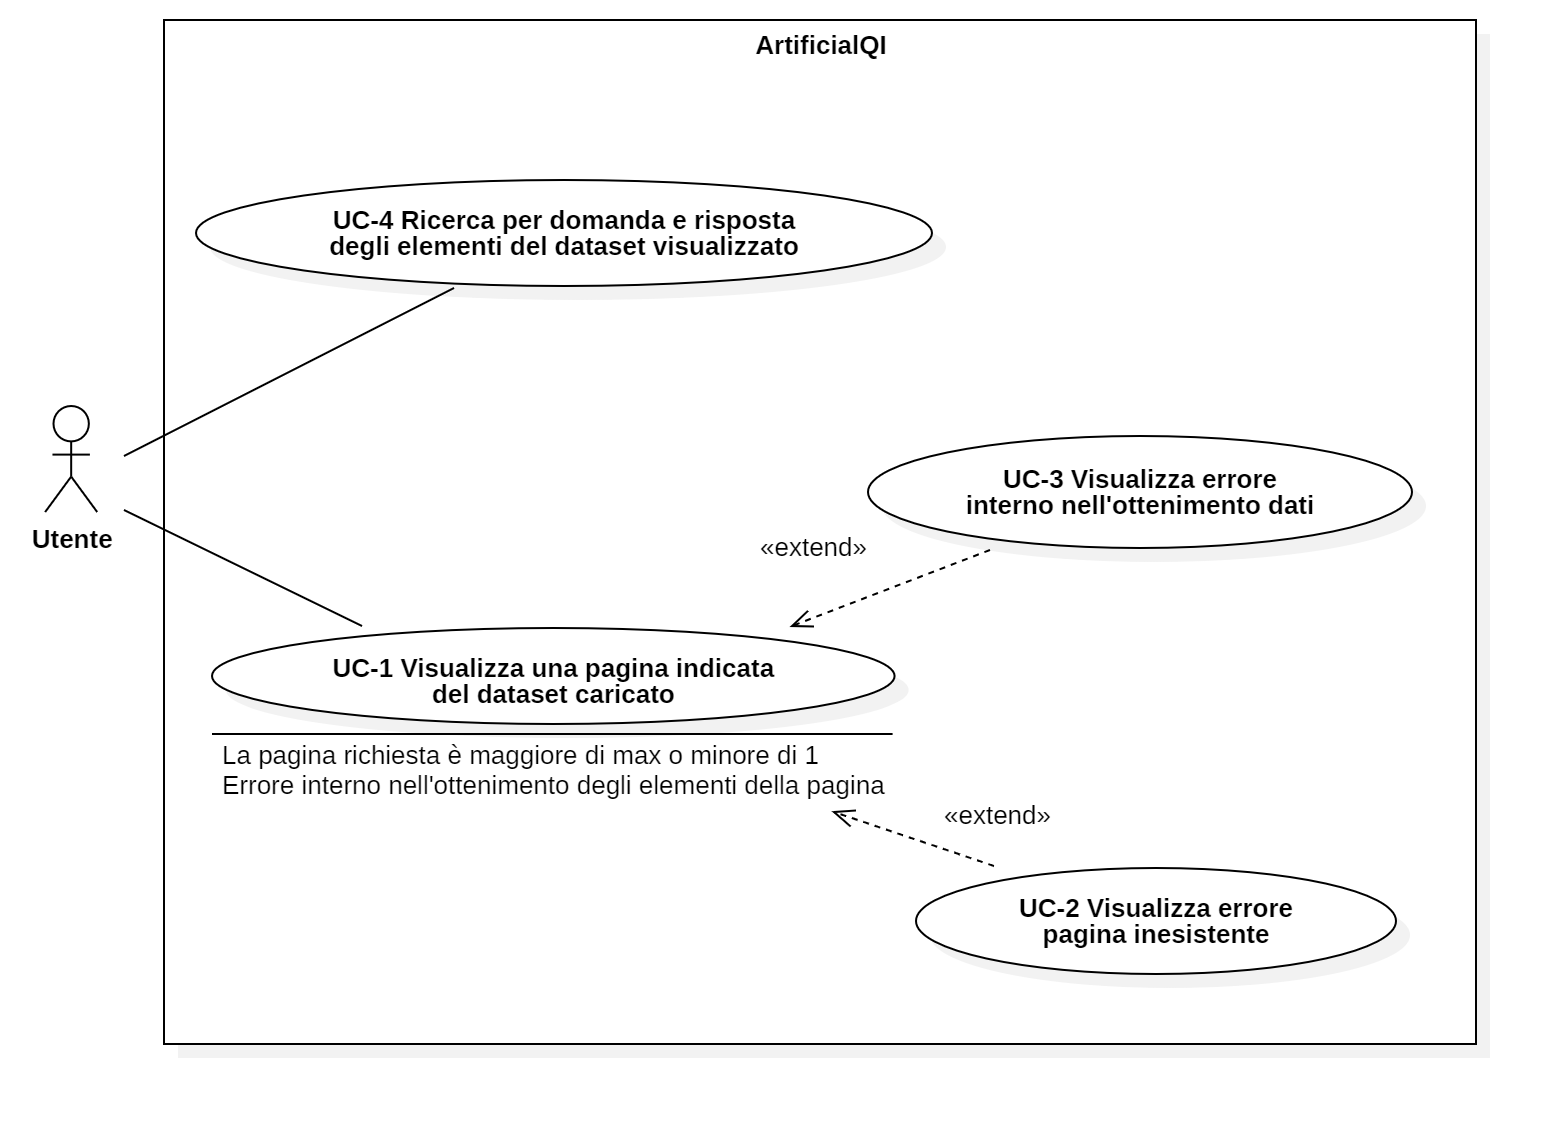
\includegraphics[scale=0.23]{Sezioni/UseCase/Immagini/VisualizzazioneDatasetCaricato}
    \caption{Diagramma visualizzazione dataset caricato.}
\end{figure}

\begin{usecase}{UC-1}{Visualizza una pagina indicata del dataset caricato}
    \label{uc:UC-1}    
    
    \req{\hyperref[ru:RUO-1]{RUO-1}} 

    \pre{
        \item L'utente ha caricato un dataset
    }

    \post{
        \item Viene visualizzata la pagina del dataset caricato indicata
    }
    
    \actor{Utente}

    \subactors{}

    \trigger{L'utente vuole visualizzare il contenuto di una pagina del dataset caricato}
    
    \inc{}

    \base{}

    \scenario{
        \item L'utente richiede la visualizzazione di una pagina del dataset caricato
        \item Il sistema verifica che il dataset caricato non sia vuoto
        \item Il sistema verifica che la pagina richiesta esista
        \item Il sistema ottiene gli elementi che compongono la pagina richiesta
        \item Gli elementi vengono visualizzati in una lista dove ogni elemento viene mostrato come una coppia domanda-risposta
    }

    \subscenario{
        \item[2.1] Il dataset caricato è vuoto:
        \begin{itemize}
            \item[a.] Viene indicato all'utente che il dataset caricato è vuoto
        \end{itemize}

        \item[3.1] La pagina richiesta non esiste ovvero è inferiore a uno o superiore alla pagina massima:
        \begin{itemize}
            \item[a.] \hyperref[uc:UC-2]{UC-2}
        \end{itemize}

        \item[4.1] Errore interno durante l'ottenimento degli elementi:
        \begin{itemize}
            \item[a.] \hyperref[uc:UC-3]{UC-3}
        \end{itemize}
        
    }
\end{usecase}

\begin{usecase}{UC-2}{Visualizza errore pagina inesistente}
    \label{uc:UC-2}
    
    \req{} 

    \pre{
        \item Il controllo di validità del numero di pagina fallisce
    }

    \post{
        \item L’utente capisce che la pagina richiesta non esiste e viene informato sull’intervallo di pagine valide
    }

    \actor{Utente}

    \subactors{}

    \trigger{Il sistema ha ricevuto una richiesta di visualizzazione per una pagina inesistente}

    \inc{}

    \base{}

    \scenario{
        \item Viene visualizzato un messaggio di errore che informa l'utente che la pagina richiesta non esiste
        \item Viene indicato il range di pagine valide 
    }

    \subscenario{}

\end{usecase}


\begin{usecase}{UC-3}{Visualizza errore interno nell'ottenimento dati}
    \label{uc:UC-3}
    
    \req{} 

    \pre{
        \item Avviene un errore interno al sistema durante l'ottenimento di uno o più dati gestiti da esso
    }

    \post{
        \item L'utente è a conoscenza dell'errore interno avvenuto
    }

    \actor{Utente}

    \subactors{}

    \trigger{Il sistema riscontra un errore interno durante l'ottenimento di dati}

    \inc{}

    \base{}

    \scenario{
        \item Viene mostrato un messaggio di errore che informa l'utente sulla natura dell'errore
    }

    \subscenario{}

\end{usecase}


\begin{usecase}{UC-4}{Ricerca per domanda e risposta degli elementi del dataset visualizzato}
    \label{uc:UC-4}
    
    \req{\hyperref[ru:RUO-2]{RUO-2}} 

    \pre{
        \item L'utente sta visualizzando una pagina del dataset caricato \hyperref[uc:UC-1]{UC-1}
    }

    \post{
        \item Vengono selezionati gli elementi che corrispondono dalla ricerca
        \item Viene visualizzata la prima pagina dei risultati
    }
    
    \actor{Utente}

    \subactors{}

    \trigger{L'utente vuole eseguire una ricerca per domanda e risposta sul dataset caricato}
    
    \inc{}

    \base{}

    \scenario{
        \item L’utente specifica le parole chiave da usare per la ricerca
        \item Il sistema ricerca gli elementi che contengono le parole chiave nella propria domanda e/o risposta
        \item Il sistema restringe internamente il dataset caricato agli elementi risultanti dalla ricerca
        \item Viene visualizzata la prima pagina dei risultati
    }

    \subscenario{}

\end{usecase}